\chapter{FUNDAMENTAÇÃO TEÓRICA} \label{cap:Fundamentacao}
% ----------------------------------------------------------
A arquitetura de software é um dos pilares centrais no desenvolvimento de sistemas computacionais modernos. Ela define a estrutura organizacional de um sistema, estabelecendo diretrizes para a disposição dos seus componentes, suas interações e restrições, além de orientar decisões técnicas que impactam diretamente na escalabilidade, manutenção e evolução do software ao longo do tempo \cite{jamshidi2016systematic}.

De acordo com \cite{jamshidi2016systematic}, a arquitetura de software pode ser compreendida como o conjunto de estruturas necessárias para raciocinar sobre o sistema, que compreende elementos de software, as relações entre eles e as propriedades de ambos. Em outras palavras, a arquitetura de software não se limita apenas à divisão do sistema em módulos, mas também envolve a definição de padrões de comunicação, protocolos, mecanismos de segurança, estratégias de escalabilidade e diretrizes para integração entre componentes. 

A definição de uma arquitetura adequada é fundamental para garantir que o sistema atenda aos requisitos funcionais e não funcionais, como desempenho, segurança, confiabilidade e facilidade de manutenção. Segundo \cite{nizami2020comparison}, a escolha da arquitetura influencia diretamente a capacidade do sistema de evoluir e se adaptar a novas demandas, sendo um fator determinante para o sucesso de projetos de software em ambientes dinâmicos e competitivos.

Historicamente, a arquitetura monolítica foi o modelo predominante no desenvolvimento de sistemas. Nesse paradigma, todas as funcionalidades do software são implementadas em um único bloco, compartilhando o mesmo ambiente de execução, banco de dados e ciclo de vida \cite{nizami2020comparison}. Essa abordagem, embora simples de implementar e gerenciar em projetos de menor escala, apresenta limitações significativas à medida que o sistema cresce, como dificuldades de manutenção, escalabilidade restrita e maior risco de falhas generalizadas. 

Com o avanço das demandas por sistemas mais flexíveis, escaláveis e resilientes, especialmente em ambientes de computação em nuvem, emergiu a arquitetura de microsserviços como uma alternativa ao modelo monolítico \cite{jamshidi2016systematic, shekhar2023microservices}. Os microsserviços propõem a fragmentação do sistema em serviços independentes, cada um responsável por uma funcionalidade específica e comunicando-se por meio de interfaces bem definidas. Essa abordagem permite que equipes distintas desenvolvam, testem e implantem serviços de forma autônoma, promovendo ciclos de entrega mais curtos e maior adaptabilidade às mudanças. 

Além disso, a arquitetura de microsserviços facilita a adoção de práticas modernas de \textit{DevOps}, automação de \textit{deploys} e escalabilidade granular, alinhando-se às necessidades de negócios que exigem respostas rápidas e contínuas às mudanças do mercado \cite{shekhar2023microservices}. No entanto, essa evolução também traz novos desafios, como a necessidade de ferramentas avançadas para orquestração, monitoramento e observabilidade, além de uma curva de aprendizado mais acentuada para as equipes de desenvolvimento \cite{jamshidi2016systematic}. 

A definição de padrões arquiteturais é essencial para garantir a organização, escalabilidade e manutenção de sistemas de software. Diversos padrões foram consolidados na literatura internacional, cada um com características, vantagens e limitações específicas \cite{jamshidi2016systematic}. 

Um dos padrões mais tradicionais é a arquitetura monolítica, na qual todas as funcionalidades do sistema são implementadas em um único bloco de código, compartilhando o mesmo ambiente de execução e banco de dados. Embora seja simples de desenvolver e implantar, esse modelo apresenta dificuldades de escalabilidade e manutenção à medida que o sistema cresce. Como afirmam \cite{nizami2020comparison}: 

“A arquitetura monolítica é fácil de desenvolver e fazer \textit{deploy}, mas, à medida que a aplicação cresce, torna-se difícil de gerenciar, escalar e manter. Qualquer pequena mudança requer que toda a aplicação seja reconstruída e reimplantada, o que aumenta o risco e o esforço.” 

Essa limitação faz com que, em projetos de maior porte, a arquitetura monolítica se torne menos atrativa, especialmente quando há necessidade de frequentes atualizações e escalabilidade do sistema. 

A arquitetura em camadas é amplamente utilizada em sistemas corporativos. Nesse modelo, o sistema é dividido em diferentes camadas, como apresentação, lógica de negócio e acesso a dados, cada uma com responsabilidades bem definidas. Essa separação facilita a manutenção, a reutilização de componentes e a evolução do sistema, além de permitir que equipes distintas trabalhem de forma mais organizada \cite{jamshidi2016systematic}. 

A \textit{Service-Oriented Architecture} (\textit{SOA}) propõe a construção de sistemas a partir de serviços independentes, que se comunicam por meio de protocolos padronizados, como \textit{REST} ou \textit{SOAP}. O \textit{SOA} foi fundamental para a integração de sistemas heterogêneos e para a criação de soluções mais flexíveis, permitindo que diferentes aplicações compartilhem funcionalidades de forma segura e controlada. No entanto, a complexidade de orquestração e a dependência de barramentos de serviço podem tornar a implementação desse padrão mais desafiadora \cite{jamshidi2016systematic}. 

Nos últimos anos, a arquitetura de microsserviços ganhou destaque, principalmente devido à sua capacidade de promover a independência entre equipes, a escalabilidade granular e a facilidade de adoção de práticas modernas de \textit{DevOps}. Cada microsserviço é responsável por uma funcionalidade específica e pode ser desenvolvido, testado, implantado e escalado de forma autônoma. Essa flexibilidade, no entanto, exige um investimento maior em ferramentas de monitoramento, orquestração e observabilidade, além de demandar uma curva de aprendizado mais acentuada para as equipes de desenvolvimento \cite{jamshidi2016systematic, shekhar2023microservices, nizami2020comparison}. 

\section{Padrões Arquiteturais}

\subsection{Arquitetura Monolítica}

A arquitetura monolítica caracteriza-se pela integração de todos os componentes funcionais do sistema - interface de usuário, lógica de negócio e acesso a dados - em uma única unidade de \textit{deploy} e execução \cite{nizami2020comparison}. Nesse modelo, o acoplamento entre módulos é extremamente elevado, uma vez que compartilham o mesmo espaço de memória, base de dados e ciclo de vida. Conforme destacado por \cite{farhan2023performance}, essa estrutura promove rapidez no desenvolvimento inicial devido à simplicidade de configuração e depuração, sendo ideal para protótipos ou sistemas com escopo limitado.

Entretanto, à medida que o sistema expande sua base de código e adquire maior complexidade, surgem desafios significativos que impactam diretamente a manutenção e a evolução da aplicação. Um dos principais entraves é a escalabilidade vertical obrigatória: a única estratégia viável consiste na replicação da aplicação inteira, mesmo quando apenas componentes específicos demandam mais recursos \cite{nizami2020comparison}. Essa limitação resulta em desperdício de recursos computacionais e aumento de custos operacionais, dificultando o crescimento sustentável do sistema.

Outro ponto crítico refere-se à rigidez tecnológica. A adoção de novas tecnologias ou versões de bibliotecas exige a atualização do monolito como um todo, o que gera \textit{lock-in} tecnológico e limita a capacidade de inovação \cite{jamshidi2016systematic}. Esse cenário dificulta a experimentação e a incorporação de soluções modernas, tornando o sistema menos adaptável às mudanças do mercado e às demandas dos usuários.

Além disso, há o comprometimento da confiabilidade. Falhas em módulos secundários podem paralisar toda a aplicação, uma vez que todos os componentes compartilham o mesmo ambiente de execução. Testes de carga realizados por \cite{farhan2023performance} demonstram que a indisponibilidade de um único módulo pode resultar em \textit{downtime} total, evidenciando a fragilidade desse modelo em relação à resiliência.

Por fim, destaca-se a complexidade evolutiva. Modificações em qualquer parte do sistema exigem reteste e reimplantação completos, ampliando os riscos e o \textit{lead time} para a entrega de novas funcionalidades. Esse processo torna-se cada vez mais oneroso à medida que o sistema cresce, dificultando a manutenção e a evolução contínua da aplicação.

\begin{figure}[H]
\centering
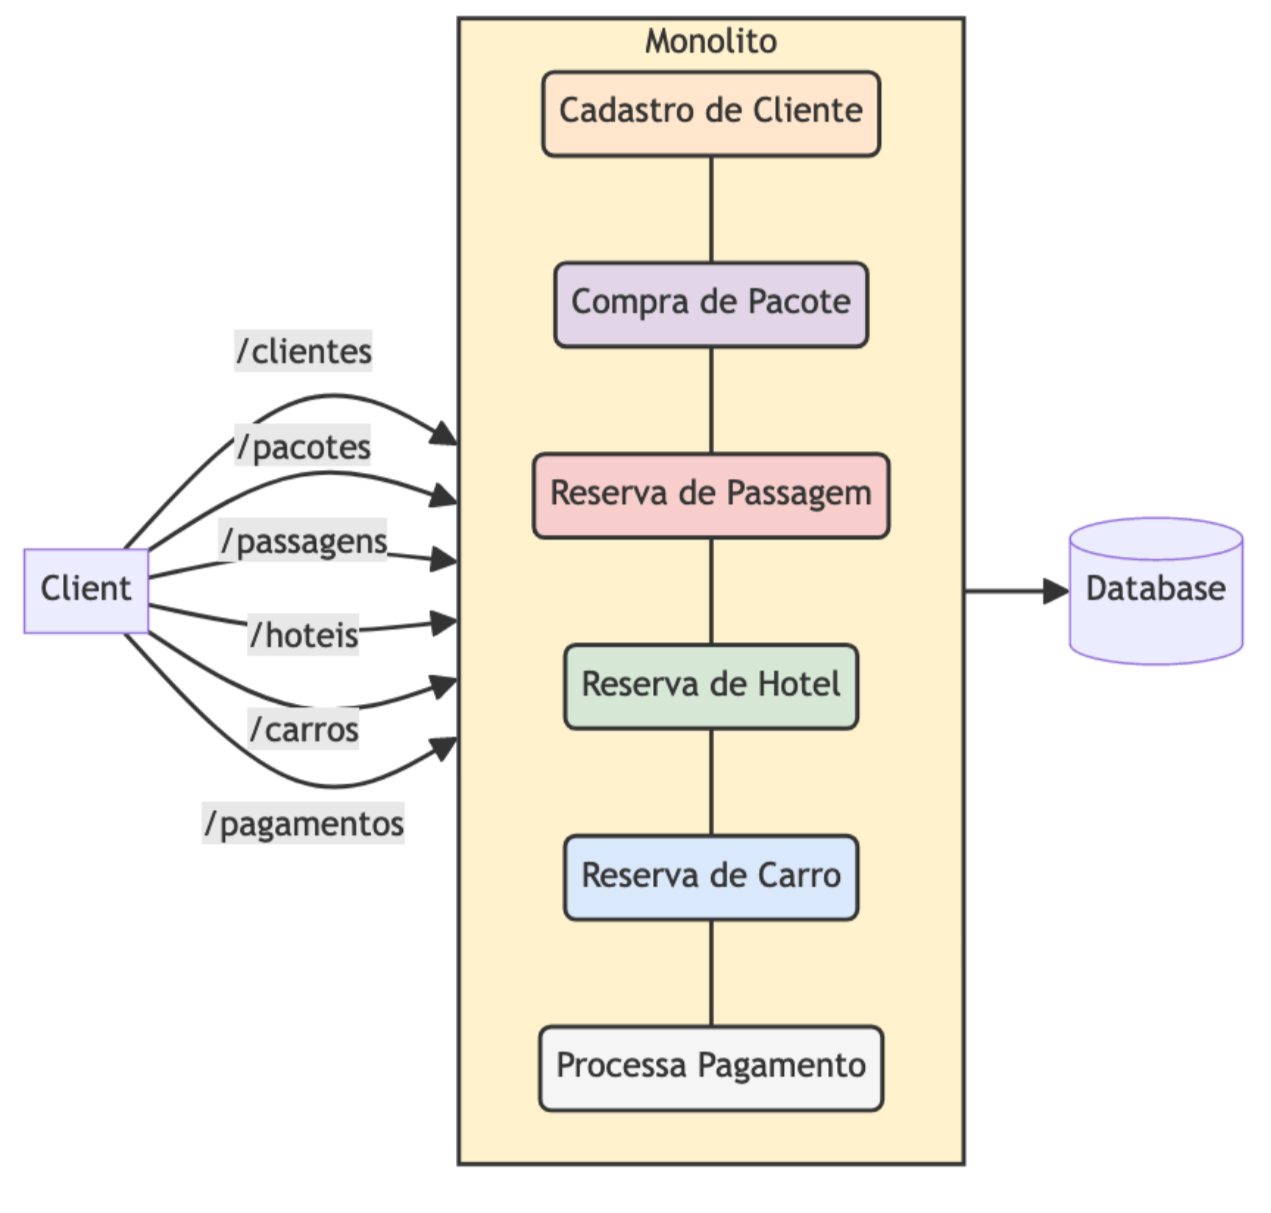
\includegraphics[width=0.8\textwidth]{images/monolito.png}
\caption{Estrutura típica de arquitetura monolítica.}
\label{fig:monolitico}
\end{figure}

Como ilustrado na Figura~\ref{fig:monolitico}, a arquitetura monolítica caracteriza-se pela centralização de todos os módulos e funcionalidades do sistema em uma única aplicação, onde as camadas como apresentação, lógica de negócio e acesso a dados encontram-se fortemente acopladas e compartilham o mesmo espaço de execução. O fluxo de requisições percorre camadas internamente acopladas, sem isolamento de processos. Essa centralização, embora simplifique o desenvolvimento inicial, apresenta limitações significativas em cenários de alta demanda e necessidade de escalabilidade.

Segundo Farhan et al.~\cite{farhan2023performance}, sistemas monolíticos apresentaram, em testes empíricos, 40\% maior tempo de resposta sob carga crescente, 68\% mais \textit{downtime} durante atualizações e limite máximo de escalonamento em cinco instâncias, devido ao compartilhamento de recursos e à ausência de isolamento entre processos. Portanto, embora a arquitetura monolítica seja adequada para aplicações de menor porte ou com requisitos estáveis, suas restrições de escalabilidade, resiliência e flexibilidade tornam-se evidentes em ambientes dinâmicos e de grande escala, justificando a busca por alternativas arquiteturais mais modernas.

Portanto, embora a arquitetura monolítica seja adequada para aplicações de menor porte ou com requisitos estáveis, suas restrições de escalabilidade, resiliência e flexibilidade tornam-se evidentes em ambientes dinâmicos e de grande escala, justificando a busca por alternativas arquiteturais mais modernas.

O fluxo de requisições percorre camadas internamente acopladas, sem isolamento de processos. Essa centralização explica os resultados empíricos de \cite{farhan2023performance}, onde sistemas monolíticos apresentaram:
O fluxo de requisições em sistemas monolíticos percorre camadas fortemente acopladas, sem qualquer tipo de isolamento entre processos. Essa centralização estrutural contribui para os resultados observados por \cite{farhan2023performance}, que identificaram um aumento de 40\% no tempo de resposta sob carga crescente, além de 68\% mais \textit{downtime} durante atualizações. Outro dado relevante é o limite máximo de escalonamento, que se restringe a cinco instâncias antes que ocorra degradação crítica do desempenho, evidenciando a dificuldade de adaptação a cenários de alta demanda.

Apesar dessas limitações, a arquitetura monolítica ainda mantém relevância em contextos específicos, como aplicações com tráfego previsível, equipes de desenvolvimento co-localizadas ou situações em que a simplicidade operacional é mais importante do que requisitos de elasticidade \cite{shekhar2023microservices}. No entanto, para sistemas empresariais modernos que exigem entrega contínua, resiliência e escalabilidade dinâmica, a viabilidade do modelo monolítico torna-se progressivamente reduzida, justificando a busca por alternativas arquiteturais mais flexíveis.

\subsection{Event-Driven Architecture}
A \textit{Event-Driven Architecture} (EDA) é um paradigma arquitetural que se destaca pela capacidade de lidar com sistemas distribuídos, dinâmicos e de alta escalabilidade, sendo especialmente recomendada para aplicações que exigem resposta em tempo real e processamento assíncrono de grandes volumes de dados \cite{jamshidi2016systematic}. Nesse modelo, os componentes do sistema frequentemente implementados como microserviços comunicam-se por meio de eventos, que representam mudanças de estado ou ocorrências relevantes no domínio da aplicação. Cada evento é transmitido por um produtor e pode ser consumido por um ou mais consumidores, promovendo o desacoplamento entre os módulos e facilitando a evolução independente de cada serviço \cite{shekhar2023microservices}.

A adoção da EDA é comum em cenários como plataformas de \textit{e-commerce}, sistemas financeiros, aplicações de \textit{streaming} e ambientes de \textit{Internet das Coisas} (IoT), onde a escalabilidade horizontal e a resiliência são requisitos críticos \cite{jamshidi2016systematic, shekhar2023microservices}. Nesses contextos, a arquitetura orientada a eventos permite que múltiplos serviços processem informações de forma paralela e reativa, reduzindo gargalos e aumentando a capacidade de resposta do sistema como um todo.

Segundo Jamshidi et al.~\cite{jamshidi2016systematic}, a EDA contribui para a redução do acoplamento entre componentes, pois os serviços não dependem diretamente uns dos outros, mas sim de eventos compartilhados por meio de um barramento ou intermediário, como um \textit{message broker}. Essa característica facilita a manutenção, a escalabilidade e a resiliência, uma vez que falhas em um serviço não necessariamente impactam os demais, desde que o barramento de eventos permaneça operacional.

No entanto, a adoção da EDA traz desafios, como a complexidade na gestão do fluxo de eventos, a necessidade de garantir a ordem e a consistência das mensagens, além do aumento da dificuldade de depuração e testes em ambientes altamente distribuídos \cite{sha2023automating}. Ainda assim, os benefícios em termos de escalabilidade, flexibilidade e resiliência tornam a arquitetura orientada a eventos uma escolha estratégica para sistemas modernos e de grande porte.

\begin{figure}[H]
    \centering
    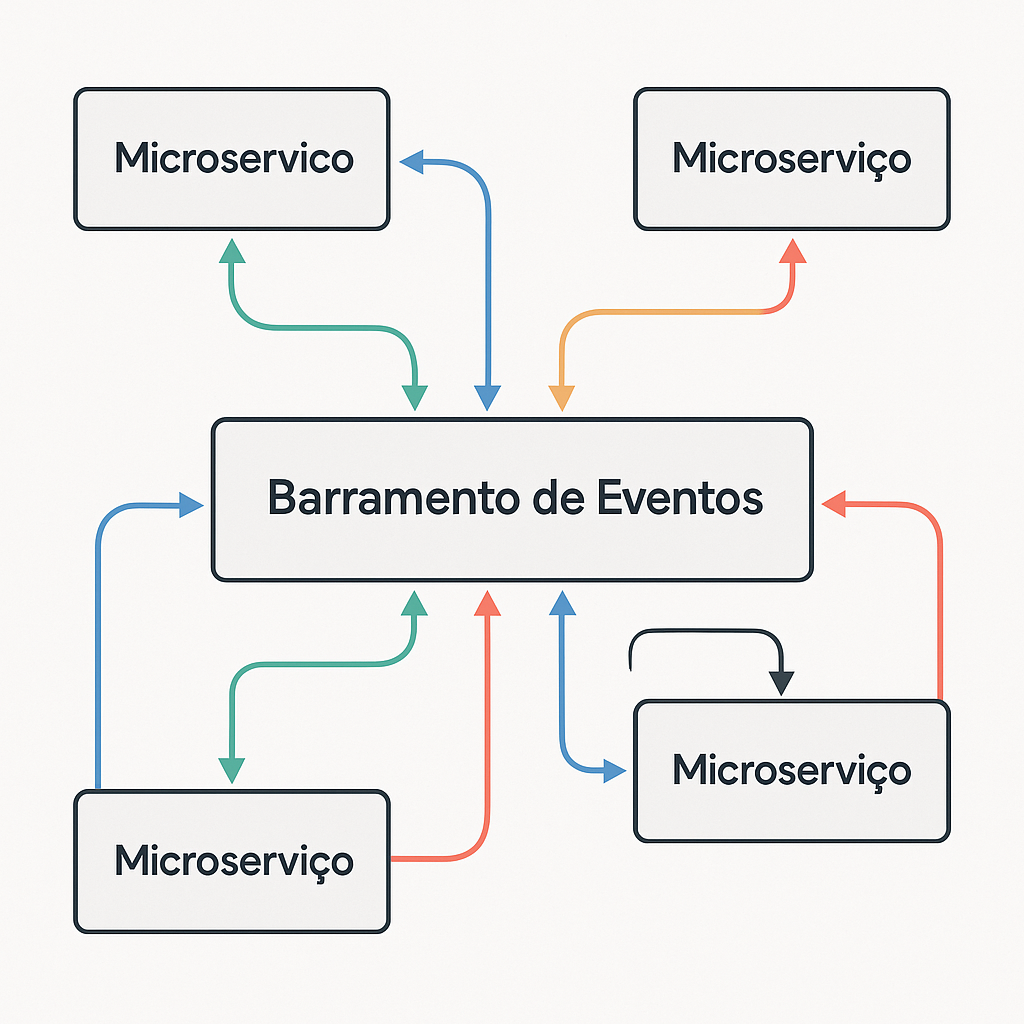
\includegraphics[width=0.7\textwidth]{images/event-driven.png}
    \caption{Arquitetura Orientada a Eventos, ilustrando a comunicação assíncrona entre microserviços através de um barramento de eventos.}
    \label{fig:event-driven}
    \parbox{\textwidth}{
        A Figura \ref{fig:event-driven} apresenta um diagrama conceitual da Arquitetura Orientada a Eventos (\textit{Event-Driven Architecture}). Nesta arquitetura, microserviços independentes comunicam-se de forma assíncrona através de um barramento de eventos central popularmente conhecido como \textit{message broker}. Os microserviços podem tanto produzir eventos, enviando-os para o barramento, quanto consumir eventos, recebendo-os do barramento. Essa abordagem promove o desacoplamento entre os serviços, facilitando a escalabilidade, a resiliência e a manutenção do sistema.
    }
\end{figure}

A Figura~\ref{fig:event-driven} apresenta um diagrama conceitual da Arquitetura Orientada a Eventos (\textit{Event-Driven Architecture}). Nesta arquitetura, microserviços independentes comunicam-se de forma assíncrona através de um barramento de eventos central popularmente conhecido como \textit{message broker}. Os microserviços podem tanto produzir eventos, enviando-os para o barramento, quanto consumir eventos, recebendo-os do barramento. Essa abordagem promove o desacoplamento entre os serviços, facilitando a escalabilidade, a resiliência e a manutenção do sistema.

\subsection{Serverless}
A arquitetura \textit{serverless} tem se destacado com o avanço das plataformas de computação em nuvem, oferecendo uma abordagem inovadora para o desenvolvimento e a execução de aplicações. Nesse modelo, os desenvolvedores podem se concentrar exclusivamente na lógica de negócio, delegando a gestão da infraestrutura ao provedor de nuvem. Essa abstração permite maior agilidade no desenvolvimento e escalabilidade automática, embora apresente desafios relacionados à portabilidade e ao controle sobre o ambiente de execução \cite{shekhar2023microservices}.

\begin{figure}[H]
\centering
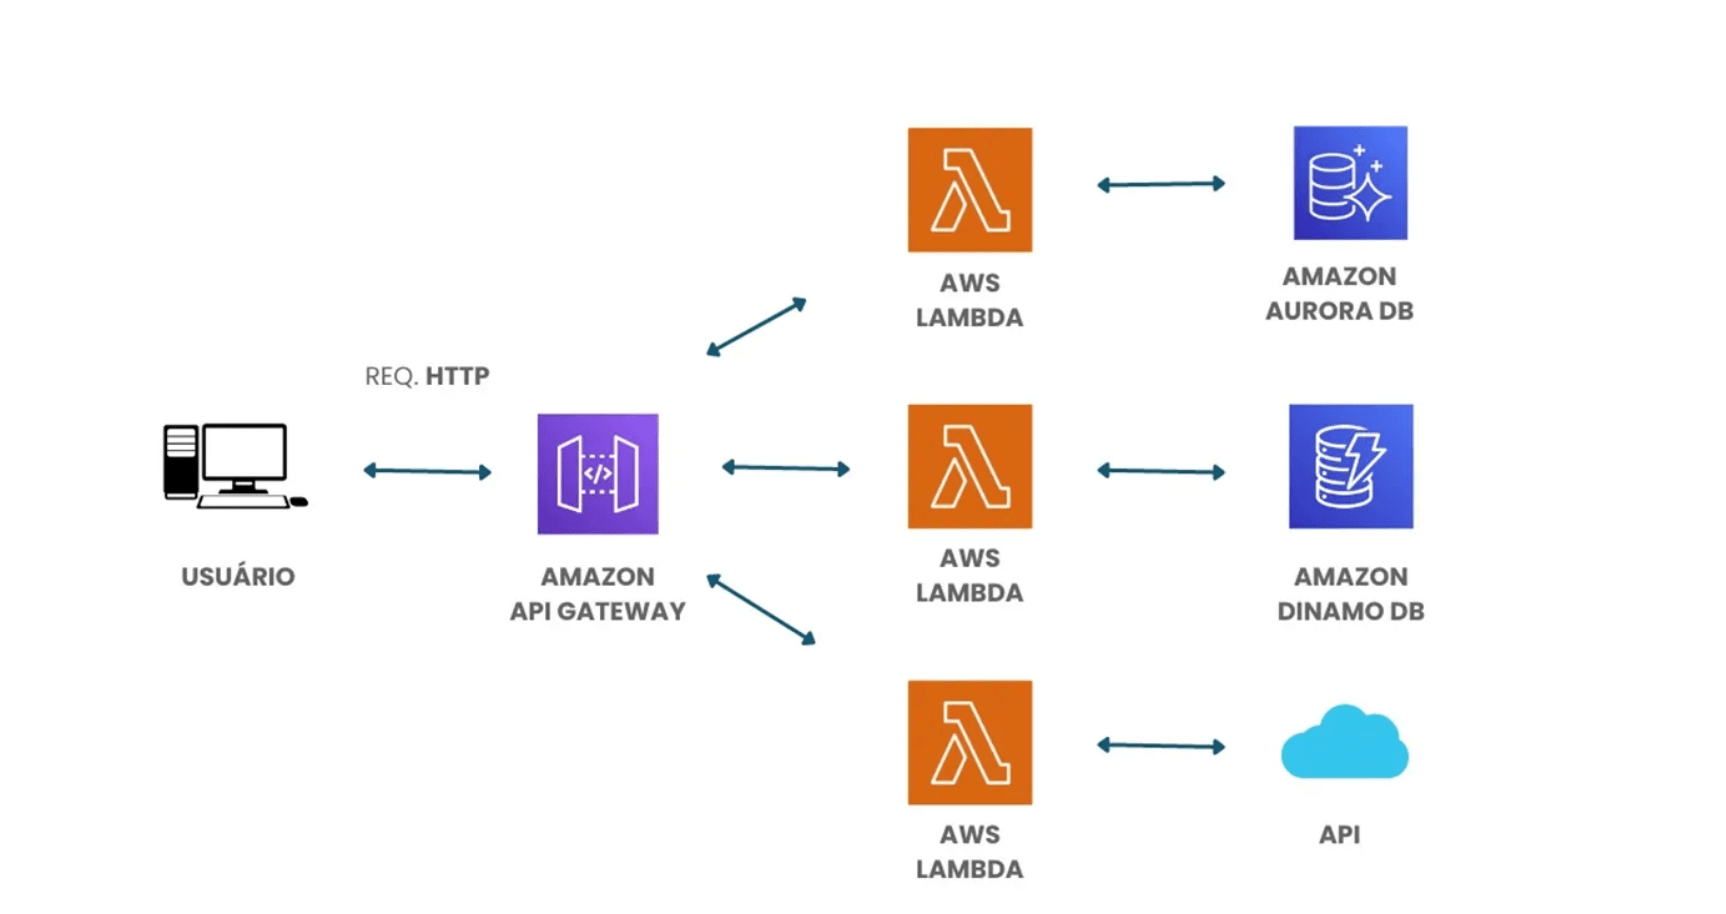
\includegraphics[width=0.9\textwidth]{images/serverless.png}
\caption{Arquitetura Serverless típica, mostrando os componentes principais: API Gateway, Funções como Serviço (FaaS), e serviços gerenciados. Fonte: Adaptado de \cite{shekhar2023microservices}.}
\label{fig:serverless}
\end{figure}

A Figura \ref{fig:serverless} ilustra um exemplo de arquitetura serverless, destacando seus componentes principais. O \textit{API Gateway} atua como o ponto de entrada único para todas as requisições, roteando o tráfego para as funções de backend. As \textit{Funções como Serviço (FaaS)}, como AWS Lambda ou Azure Functions, permitem a execução de código sob demanda, sem a necessidade de provisionar ou gerenciar servidores. Além disso, a arquitetura serverless utiliza \textit{Serviços Gerenciados}, como bancos de dados e filas de mensagens, que são providos e mantidos pelo provedor de nuvem, simplificando ainda mais a operação e a manutenção da aplicação.

A adoção do padrão serverless elimina a necessidade de gerenciamento de servidores, permitindo que os desenvolvedores foquem exclusivamente na implementação da lógica de negócios \cite{shekhar2023microservices}. A escolha do padrão arquitetural mais adequado depende de fatores como requisitos do sistema, contexto de negócio, equipe envolvida e recursos disponíveis. Compreender as vantagens e limitações de cada abordagem é essencial para alinhar a arquitetura às necessidades presentes e futuras do projeto \cite{jamshidi2016systematic, nizami2020comparison}.

\subsection{Microsserviços}
Como abordado anteriormente, a arquitetura de microsserviços decompõe sistemas em serviços autônomos. Sua implementação prática demanda atenção a três dimensões críticas: comunicação, observabilidade e orquestração. \cite{jamshidi2016systematic, nizami2020comparison}. 

Entre os principais benefícios dos microsserviços está a escalabilidade granular, que permite dimensionar apenas os serviços que realmente demandam mais recursos, otimizando custos e desempenho \cite{shekhar2023microservices}. Além disso, a independência entre equipes é favorecida, pois times distintos podem desenvolver, testar e implantar serviços de forma autônoma, acelerando o ciclo de entrega e facilitando a adoção de práticas \textit{DevOps} \cite{nizami2020comparison, farhan2023performance}.

Outro ponto relevante é a resiliência: falhas em um serviço tendem a ser isoladas, reduzindo o impacto sobre o sistema como um todo \cite{farhan2023performance}. Isso é especialmente importante em ambientes de missão crítica, onde a disponibilidade contínua é fundamental. Para garantir essa resiliência, padrões como o \textit{Circuit Breaker} são frequentemente empregados.

A observabilidade em microsserviços demanda o uso de ferramentas especializadas para coleta e análise de métricas, logs e rastreamento distribuído \cite{observability2023, sha2023automating}. Essa visibilidade é indispensável para identificar gargalos, diagnosticar falhas e garantir a saúde do sistema em produção. Soluções como Prometheus e Jaeger são amplamente utilizadas para monitorar o desempenho e rastrear o fluxo de requisições entre serviços, facilitando a manutenção e a evolução contínua da arquitetura.

Outro ponto relevante é a resiliência: falhas em um serviço tendem a ser isoladas, reduzindo o impacto sobre o sistema como um todo \cite{farhan2023performance}. Isso é especialmente importante em ambientes de missão crítica, onde a disponibilidade contínua é fundamental. Para garantir essa resiliência, padrões como o \textit{Circuit Breaker} são frequentemente empregados.

Por fim, a orquestração de microsserviços envolve o gerenciamento automatizado de implantação, escalonamento e atualização dos serviços, frequentemente utilizando plataformas como Kubernetes \cite{shekhar2023microservices}. Essa abordagem permite maior resiliência operacional, reduz o tempo de indisponibilidade e simplifica a administração de ambientes complexos. A automação dos processos de entrega contínua e recuperação de falhas é um dos pilares para o sucesso de arquiteturas baseadas em microsserviços.

\begin{figure}[H]
\centering
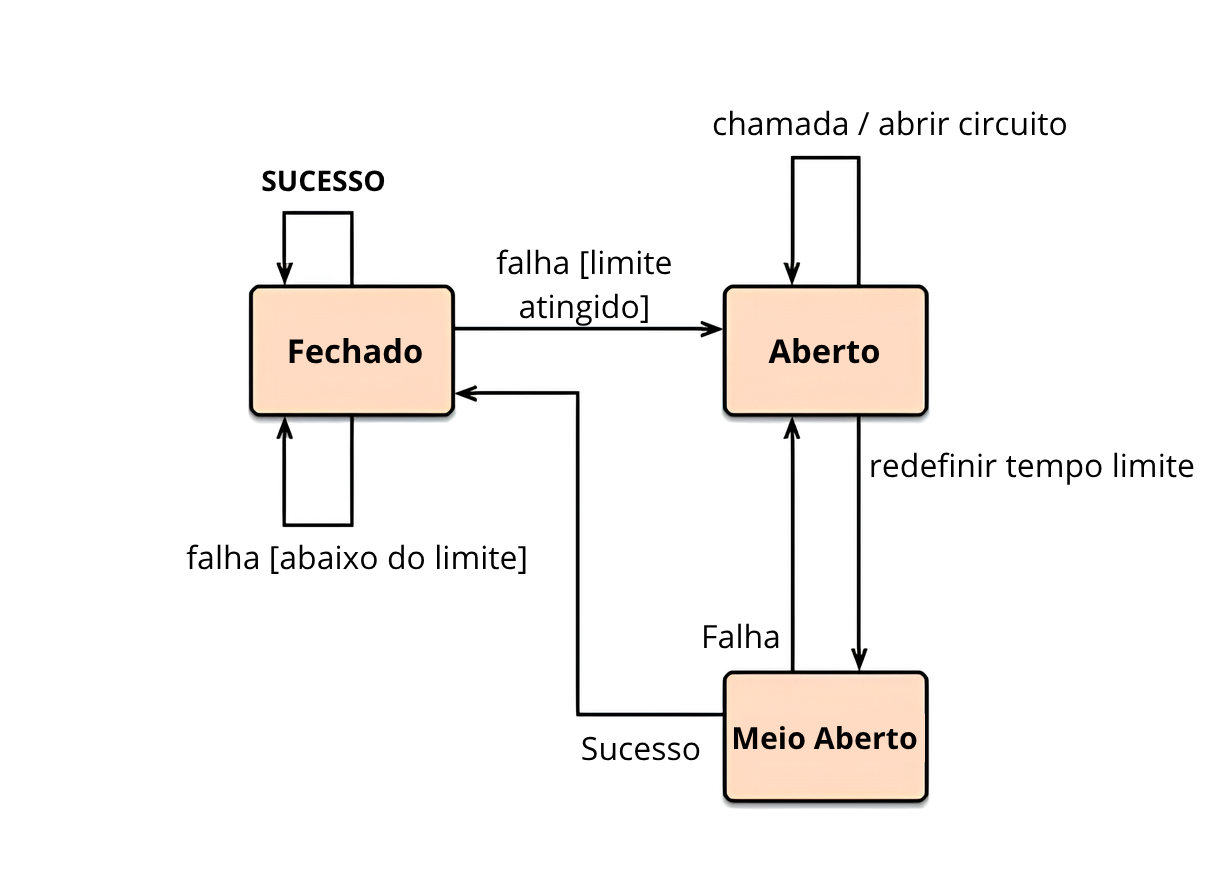
\includegraphics[width=0.7\textwidth]{./images/circuit_breaker.png}
\caption{Funcionamento do padrão Circuit Breaker em sistemas distribuídos.}
\label{fig:circuit-breaker}
\end{figure}

O \textit{Circuit Breaker} é um padrão arquitetural amplamente utilizado em sistemas distribuídos para aumentar a resiliência e evitar falhas em cascata \cite{Nair2019CircuitBreaker, Fowler2012CircuitBreaker}. Ele atua como um "interruptor" que monitora as chamadas a um serviço externo. Seu funcionamento é dividido em três estados principais: fechado, aberto e meio-aberto.

No estado fechado, todas as requisições são encaminhadas normalmente ao serviço. Se o número de falhas ultrapassar um limite configurado, o circuito entra no estado aberto, bloqueando novas tentativas e retornando imediatamente uma resposta de erro ou acionando um mecanismo de \textit{fallback} uma solução alternativa, como dados em cache ou uma resposta padrão, para manter a aplicação funcionando de forma degradada. Após um tempo de espera, o circuito passa para o estado meio-aberto, permitindo algumas requisições de teste. Se essas requisições forem bem-sucedidas, o circuito retorna ao estado fechado; caso contrário, volta ao estado aberto, protegendo o sistema de sobrecarga e falhas sucessivas \cite{Nair2019CircuitBreaker, Fowler2012CircuitBreaker}.

Esse padrão é fundamental para garantir a robustez de sistemas baseados em microsserviços, pois impede que falhas em um serviço se propaguem e comprometam toda a aplicação. Estudos recentes destacam a importância do \textit{Circuit Breaker} em arquiteturas resilientes, especialmente em ambientes de alta disponibilidade e missão crítica \cite{Nair2019CircuitBreaker}. 

No entanto, a adoção de microsserviços também traz desafios consideráveis. A complexidade operacional aumenta, exigindo ferramentas avançadas para orquestração (como \textit{Kubernetes}), monitoramento e observabilidade \cite{jamshidi2016systematic, shekhar2023microservices}. Cada serviço pode demandar sua própria infraestrutura, banco de dados e mecanismos de autenticação, o que eleva a sobrecarga de gerenciamento \cite{nizami2020comparison}.

A observabilidade torna-se um aspecto central, pois a identificação e resolução de falhas em sistemas distribuídos requerem coleta e análise de métricas, \textit{logs} e \textit{traces} distribuídos \cite{observability2023, sha2023automating}. Ferramentas como \textit{Prometheus} e \textit{Jaeger} são amplamente utilizadas para monitorar o desempenho e rastrear requisições entre serviços, facilitando o diagnóstico de problemas e a manutenção da qualidade do sistema \cite{ahmed2022observability}. 

Além disso, a escolha dos protocolos de comunicação entre microsserviços (\textit{\gls{REST}}, \textit{\gls{gRPC}}, \textit{\gls{GraphQL}}) impacta diretamente o desempenho, a flexibilidade e a observabilidade do sistema \cite{niswar2023performance}. Estudos recentes destacam que decisões arquiteturais bem fundamentadas são essenciais para garantir a eficiência e a robustez de sistemas baseados em microsserviços \cite{niswar2023performance, sha2023automating}. 

A arquitetura de microsserviços representa uma evolução paradigmática no desenvolvimento de software, decompondo sistemas complexos em serviços autônomos especializados. Conforme \cite{jamshidi2016systematic}, esta abordagem oferece:

\begin{itemize}
    \item Autonomia tecnológica: Cada serviço pode utilizar linguagens e tecnologias distintas (Java, Python, Node.js)
    \item Resiliência aprimorada: Isolamento de falhas através de padrões como \textit{Circuit Breaker}
    \item Entrega contínua: \textit{Deploys} independentes permitindo múltiplas implantações diárias
\end{itemize}

\subsubsection{Mecanismos de Comunicação}
A comunicação entre serviços em arquiteturas de microsserviços pode ser realizada por diferentes mecanismos, cada um com características, vantagens e limitações específicas. A escolha do protocolo de comunicação é um fator determinante para o desempenho, a escalabilidade e a complexidade do sistema, influenciando diretamente a experiência do usuário e a eficiência operacional \cite{niswar2023performance, maso2024comparativo}.

\begin{table}[H]
\centering
\caption{Comparação de protocolos de comunicação}
\begin{tabular}{|l|c|c|c|}
\hline
Protocolo & Latência & Complexidade & Casos de Uso \\
\hline
REST/HTTP & Alta & Baixa & Sistemas com baixa frequência \\
gRPC & Baixa & Média & Microserviços acoplados \\
Eventos (Kafka) & Assíncrona & Alta & Sistemas escaláveis \\
\hline
\end{tabular}
\label{tab:protocolos}
\end{table}

Conforme demonstrado na Tabela~\ref{tab:protocolos}, a seleção do protocolo de comunicação deve considerar o perfil de uso e os requisitos de cada aplicação. O protocolo REST/HTTP é amplamente adotado devido à sua simplicidade e compatibilidade com diferentes plataformas, sendo indicado para cenários em que a frequência de requisições não é elevada e a interoperabilidade é prioridade \cite{fielding2000rest, aws:1}. Por outro lado, o gRPC destaca-se pela baixa latência e eficiência na serialização de dados, tornando-se uma escolha adequada para integrações entre microsserviços que exigem alto desempenho e comunicação síncrona \cite{niswar2023performance, ibm:7}.

Já os mecanismos baseados em eventos, como o uso de filas e \textit{brokers} (exemplo: Kafka), possibilitam comunicação assíncrona e desacoplamento entre os serviços, favorecendo a escalabilidade horizontal e a resiliência do sistema \cite{jamshidi2016systematic, shekhar2023microservices}. Essa abordagem é especialmente recomendada para sistemas que processam grandes volumes de dados ou que demandam alta disponibilidade, pois permite que os serviços operem de forma independente, reduzindo o risco de falhas em cascata.

Além dos aspectos técnicos, a complexidade de implementação e manutenção também deve ser considerada. Protocolos como REST tendem a ser mais simples de configurar e depurar, enquanto soluções baseadas em eventos exigem infraestrutura adicional e monitoramento especializado para garantir a integridade e a ordem das mensagens \cite{maso2024comparativo, observability2023}. Dessa forma, a decisão sobre o mecanismo de comunicação deve ser pautada por uma análise criteriosa das necessidades do projeto, visando sempre o equilíbrio entre desempenho, escalabilidade e simplicidade operacional.

\subsubsection{Padrões Arquiteturais Essenciais}
\begin{figure}[H]
\centering
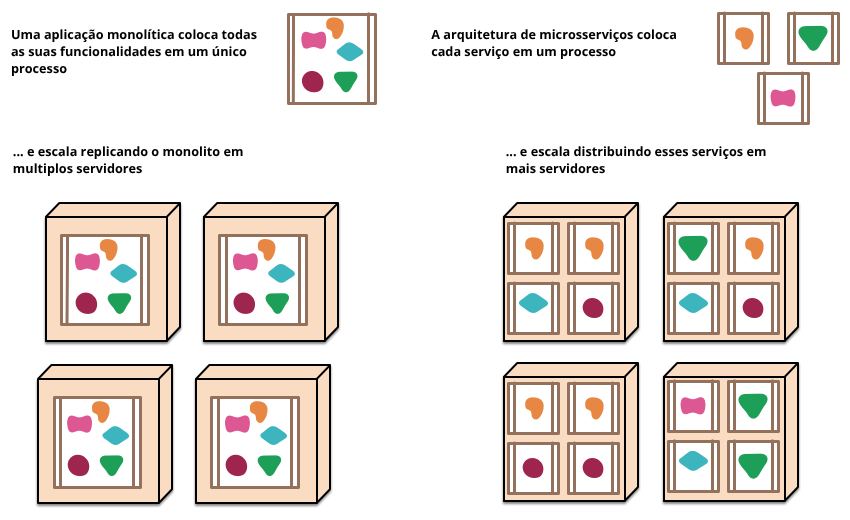
\includegraphics[width=0.7\textwidth]{images/microservice.png}
\caption{Padrões fundamentais em arquitetura de microsserviços}
\label{fig:micro_patterns}
\end{figure}

A Figura \ref{fig:micro_patterns} ilustra as diferenças fundamentais entre a arquitetura monolítica e a arquitetura de microsserviços. À esquerda, observa-se que uma aplicação monolítica agrupa todas as funcionalidades em um único processo. Para escalar esse modelo, é necessário replicar toda a aplicação em múltiplos servidores, o que pode gerar desperdício de recursos e limitações de flexibilidade.

À direita, a arquitetura de microsserviços distribui cada funcionalidade em processos independentes, permitindo que cada serviço seja desenvolvido, implantado e escalado separadamente. Isso proporciona maior eficiência no uso de recursos, facilita a manutenção e possibilita o crescimento gradual do sistema conforme a demanda por funcionalidades específicas.

Essa abordagem modular e distribuída é um dos pilares das arquiteturas modernas voltadas à escalabilidade, resiliência e agilidade no desenvolvimento.

\subsubsection{Desafios Operacionais e Soluções}
A implementação prática enfrenta obstáculos significativos:

\begin{itemize}
    \item Observabilidade: Requer integração de métricas, \textit{logs} e \textit{traces} com ferramentas como:
    \begin{itemize}
        \item \textit{Prometheus} para monitoramento
        \item \textit{Jaeger} para rastreamento distribuído
        \item \textit{EFK Stack} (Elasticsearch, Fluentd, Kibana) para análise
    \end{itemize}
    
    \item Orquestração: Plataformas como \textit{Kubernetes} gerenciam:
    \begin{itemize}
        \item Escalonamento automático
        \item Balanceamento de carga
        \item Recuperação de falhas
    \end{itemize}
\end{itemize}

\subsubsection{Melhores Práticas de Implementação}
Experiências de empresas líderes revelam estratégias eficazes:

\begin{itemize}
    \item Amazon: Utiliza a prática do "time da pizza de dois" equipes pequenas e independentes, responsáveis por serviços autônomos do início ao fim.
    
    \item Netflix: Introduziu a cultura do \textit{Chaos Engineering}, simulando falhas em produção para garantir a resiliência dos serviços.

    \item Spotify: Estruturou suas equipes em \textit{squads} responsáveis por domínios funcionais, promovendo independência e entrega contínua.

    \item Uber: Implementou uma hierarquia de serviços baseada em criticidade, diferenciando serviços centrais de auxiliares para otimizar a operação.
\end{itemize}

\subsubsection{Casos de Estudo Relevantes}
Resultados empíricos demonstram impactos mensuráveis:

\begin{table}[h]
\centering
\caption{Impacto da migração para microsserviços}
\begin{tabular}{|l|c|c|}
\hline
Métrica & Antes & Depois \\
\hline
Tempo de entrega & 30 dias & 2 dias \\
Disponibilidade & 92\% & 99.95\% \\
Custo de infraestrutura & \$100k/mês & \$65k/mês \\
\hline
\end{tabular}
\label{tab:impacto}
\end{table}

Conforme dados na Tabela \ref{tab:impacto}, organizações reportam melhorias significativas após transição bem-sucedida \cite{farhan2023performance, shekhar2023microservices}.

\subsubsection{Recomendações Estratégicas}
A adoção deve considerar:

\begin{itemize}
    \item Pré-requisitos: Maturidade em DevOps e cultura de automação
    \item Critérios: Complexidade sistêmica > 50k LOC > 15 desenvolvedores
    \item Alternativas: Arquiteturas híbridas para transição gradual
    \item Anti-padrões: Decomposição excessiva ("nanoserviços")
\end{itemize}

Em síntese, microsserviços oferecem vantagens transformacionais para sistemas complexos, mas exigem investimento proporcional em automação e governança \cite{nizami2020comparison, observability2023}.

\subsection{Protocolos de Comunicação para Microsserviços}
A seleção de protocolos de comunicação é um fator crítico em arquiteturas de microsserviços, influenciando diretamente o desempenho, acoplamento e capacidade de evolução do sistema. Dois padrões predominantes neste contexto são \gls{REST} e \gls{gRPC}, cada um com características técnicas distintas que os tornam adequados a cenários específicos \cite{niswar2023performance}.

\subsubsection{\texorpdfstring{\gls{REST}}{REST} (Representational State Transfer)}
O \gls{REST}, formalizado por Fielding \cite{fielding2000rest} em sua tese seminal, é um estilo arquitetural baseado em princípios de recursos identificáveis por \gls{URI} e operações padronizadas via verbos \gls{HTTP} (GET, POST, PUT, DELETE). Sua adoção generalizada deve-se a:

\begin{itemize}
    \item Simplicidade: Utiliza formatos legíveis como \gls{JSON}, facilitando a depuração e a integração entre sistemas heterogêneos. No entanto, a serialização textual pode consumir de 30\% a 50\% mais banda em comparação com protocolos binários \cite{niswar2023performance}.
    \item \textit{Stateless}: Cada requisição carrega todo o contexto necessário, eliminando a necessidade de manter estado no servidor e favorecendo a escalabilidade horizontal \cite{fielding2000rest}.
    \item Interface Uniforme: Princípios como a identificação única de recursos via URI e o uso de HATEOAS (\textit{Hypermedia as the Engine of Application State}) garantem consistência e desacoplamento. Com HATEOAS, as respostas da API incluem hipermídia (links) que orientam o cliente sobre as próximas ações possíveis, promovendo navegação dinâmica e reduzindo o acoplamento entre cliente e servidor \cite{maso2024comparativo}.
    \item Compatibilidade: Possui suporte nativo em navegadores e ampla adoção em APIs públicas, facilitando a integração com diferentes plataformas \cite{maso2024comparativo}.
\end{itemize}

Limitações em cenários complexos:
\begin{itemize}
\item Overhead de comunicação: Serialização textual aumenta latência e consumo de \gls{CPU}, especialmente em payloads grandes \cite{niswar2023performance}.
\item Modelo síncrono: Suporta apenas comunicação unária (request/response), inviabilizando fluxos assíncronos \cite{niswar2023performance}.
\item Falta de contratos rígidos: Validação de esquemas depende de implementações adicionais \cite{maso2024comparativo}.
\end{itemize}

Operações Básicas e Códigos HTTP:
A Tabela \ref{tab:rest_operations} sintetiza o mapeamento CRUD em REST, conforme padrões industriais \cite{fielding2000rest}:

\begin{table}[h]
\centering
\caption{Operações REST e códigos HTTP}
\label{tab:rest_operations}
\begin{tabular}{|l|c|c|}
\hline
Método HTTP & Ação & Código Sucesso \\ \hline
GET & Ler recurso & 200 (OK) \\ \hline
POST & Criar recurso & 201 (Created) \\ \hline
PUT/PATCH & Atualizar recurso & 200 (OK) ou 204 (No Content) \\ \hline
DELETE & Excluir recurso & 204 (No Content) \\ \hline
\end{tabular}
\fonte{Adaptado de \cite{niswar2023performance} e \cite{fielding2000rest}.}
\end{table}

A adoção do REST em arquiteturas de microsserviços proporciona diversos benefícios, especialmente pela padronização da comunicação e pela facilidade de integração entre componentes heterogêneos. O uso de URIs para identificação de recursos, aliado à interface uniforme baseada em métodos HTTP, simplifica o desenvolvimento e a manutenção dos serviços, permitindo que diferentes equipes trabalhem de forma independente e escalável \cite{fielding2000rest, maso2024comparativo}.

Além disso, a independência de estado (\textit{stateless}) facilita o balanceamento de carga e a replicação dos serviços, pois qualquer instância do servidor pode processar requisições sem depender de informações armazenadas em sessões. Essa característica é fundamental para ambientes distribuídos e de alta disponibilidade, comuns em sistemas modernos baseados em microsserviços.

Por outro lado, é importante considerar que, apesar de sua simplicidade e ampla adoção, o REST pode apresentar limitações em cenários que exigem comunicação em tempo real, operações transacionais complexas ou validação rígida de contratos. Nesses casos, pode ser necessário complementar a arquitetura com outros padrões ou protocolos, como gRPC ou eventos assíncronos, para atender a requisitos específicos de desempenho e flexibilidade \cite{niswar2023performance}.

Dessa forma, a arquitetura REST permanece como uma das principais escolhas para a construção de APIs robustas, escaláveis e de fácil integração, sendo amplamente utilizada tanto em aplicações web quanto em ambientes de microsserviços.

\begin{figure}[H]
    \centering
    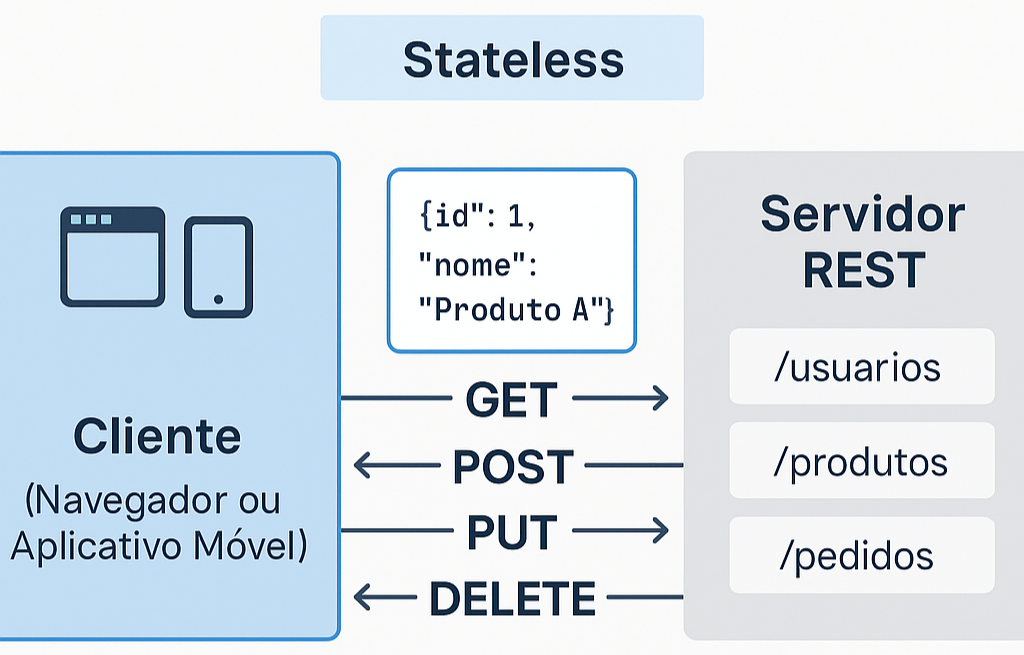
\includegraphics[width=0.7\textwidth]{images/rest.png}
    \caption{Arquitetura REST: comunicação stateless entre cliente e servidor, utilizando métodos HTTP (GET, POST, PUT, DELETE) para manipulação de recursos identificados por URI. O diagrama destaca os princípios REST, exemplos de URIs e resposta JSON, evidenciando a interface uniforme e a ausência de estado.}
    \label{fig:rest-arquitetura}
\end{figure}

A Figura~\ref{fig:rest-arquitetura} ilustra a arquitetura REST, evidenciando a troca de mensagens entre cliente e servidor por meio de métodos HTTP padronizados. Os recursos são identificados por URIs específicas, e as respostas são geralmente estruturadas em formato JSON. O princípio stateless garante que cada requisição seja independente, promovendo escalabilidade e simplicidade na integração entre sistemas.

\subsubsection{gRPC (gRPC Remote Procedure Calls)}

O \gls{gRPC} é um \textit{framework} aberto de alta performance para chamadas de procedimento remoto (RPC), desenvolvido pelo Google e lançado em 2015, que utiliza \gls{HTTP/2} e \textit{Protocol Buffers} para comunicação binária eficiente \cite{niswar2023performance, maso2024comparativo}. Sua adoção em arquiteturas de microsserviços deve-se a diferenciais como desempenho superior, suporte a streaming bidirecional, contratos fortemente tipados e geração automática de código.

\begin{itemize}
    \item Desempenho superior: A serialização binária via \textit{Protocol Buffers} reduz o tamanho dos \textit{payloads} e a latência em relação a APIs REST tradicionais, conforme mensurações em ambientes controlados \cite{niswar2023performance}.
    \item Streaming bidirecional: Suporte nativo a fluxos contínuos de dados (cliente-servidor, servidor-cliente e bidirecional), habilitando comunicação assíncrona para aplicações em tempo real \cite{maso2024comparativo}.
    \item Contratos fortemente tipados: Definição explícita de serviços e estruturas de mensagens em arquivos \texttt{.proto}, garantindo compatibilidade e evolução controlada de APIs \cite{shekhar2023microservices}.
    \item Geração de código automática: Compilação de \textit{stubs} clientes e servidores em múltiplas linguagens de programação a partir de arquivos \texttt{.proto}, promovendo consistência e redução de erros \cite{shekhar2023microservices}.
\end{itemize}

Apesar das vantagens, alguns desafios são observados:
\begin{itemize}
    \item Acoplamento forte: Alterações nos contratos \texttt{.proto} exigem atualização sincronizada de clientes e servidores, aumentando a complexidade de evolução em sistemas distribuídos \cite{shekhar2023microservices}.
    \item Curva de aprendizagem: A definição de contratos e manipulação de fluxos de \textit{streaming} pode ser complexa, especialmente para desenvolvedores familiarizados com paradigmas REST \cite{maso2024comparativo}.
\end{itemize}

A Figura~\ref{fig:grpc_streaming} apresenta os quatro padrões de comunicação suportados pelo gRPC, cada um adequado a diferentes cenários de integração entre serviços distribuídos.

\begin{figure}[H]
    \centering
    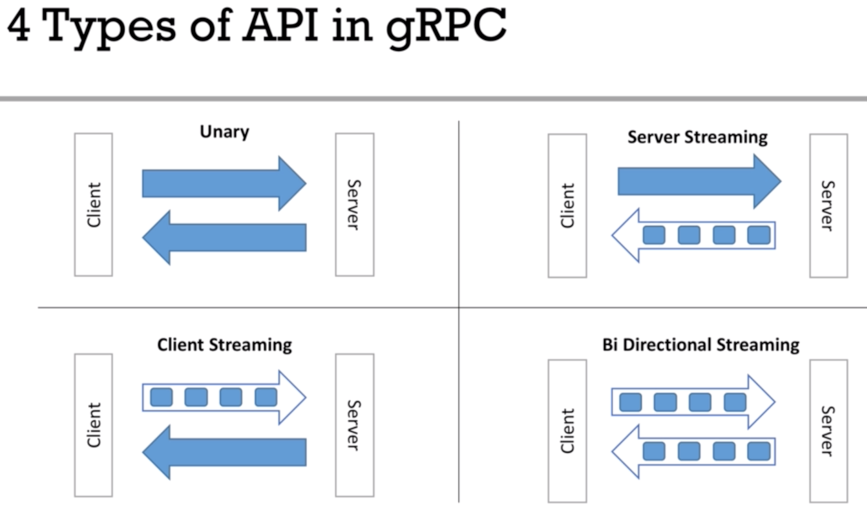
\includegraphics[width=1.0\textwidth]{images/grpc.png}
    \caption{Padrões de streaming no gRPC: (A) Unário, (B) Servidor, (C) Cliente, (D) Bidirecional.}
    \label{fig:grpc_streaming}
\end{figure}

No padrão \textit{unary} (A), o cliente realiza uma chamada simples, enviando uma única requisição ao servidor e recebendo uma única resposta. Esse modelo é o mais próximo das operações tradicionais de APIs REST, sendo indicado para transações pontuais e de baixa complexidade, como consultas ou comandos diretos.

O padrão \textit{server streaming} (B) ocorre quando o cliente envia uma requisição e o servidor responde com um fluxo contínuo de mensagens. Esse padrão é útil em situações em que o servidor precisa retornar uma grande quantidade de dados ou fornecer atualizações progressivas, como em relatórios extensos ou notificações em tempo real.

No padrão \textit{client streaming} (C), o cliente envia um fluxo de mensagens ao servidor, que processa todas as informações recebidas e retorna uma única resposta ao final. Esse modelo é apropriado para cenários em que múltiplos dados precisam ser enviados de forma agrupada, como uploads de arquivos ou envio de lotes de registros.

Por fim, o padrão \textit{bidirectional streaming} (D) permite que tanto o cliente quanto o servidor enviem múltiplas mensagens de forma independente e assíncrona, compartilhando um canal de comunicação contínuo. Esse padrão é especialmente poderoso para aplicações que exigem troca dinâmica de dados em tempo real, como chats, jogos online ou monitoramento de sensores, proporcionando máxima flexibilidade e desempenho na comunicação entre microsserviços \cite{niswar2023performance, shekhar2023microservices}.

Vantagens Técnicas Comprovadas: Estudos empíricos demonstram ganhos operacionais mensuráveis \cite{niswar2023performance}:
\begin{itemize}
    \item Redução de 35-45\% no consumo de CPU durante serialização;
    \item Até 7x maior throughput em comunicações inter-serviços.
\end{itemize}
% \ref{cap:Introducao}).
% \ref{cap:Introducao}).
% % ----------------------------------------------------------
% \section{CONCEITOS EXPLORADOS NO TRABALHO}\label{sec:conceitos}
% % ----------------------------------------------------------

% Para cada conceito explorado no trabalho, você deve criar nova uma seção como esta, por exemplo: “2.1 INTERNET DAS COISAS”.

% % ----------------------------------------------------------
% \section{TECNOLOGIAS UTILIZADAS NO DESENVOLVIMENTO}\label{sec:tecnologias}
% % ----------------------------------------------------------

% Para cada tecnologia utilizada no desenvolvimento, você deve criar uma nova seção como esta, por exemplo: “2.2 PLATAFORMA ARDUINO”.

% ----------------------------------------------------------
% \section{Exemplo citação longa em Látex} \label{}
% ----------------------------------------------------------


% \begin{citacao}
% 	Após a ilustração, na parte inferior, indicar a fonte consultada (elemento obrigatório, mesmo que seja produção do próprio autor), legenda, notas e outras informações necessárias à sua compreensão (se houver). A ilustração deve ser citada no texto e inserida o mais próximo possível do texto a que se refere. \cite[p. 11]{gil2008metodos}.
% \end{citacao}

% % ----------------------------------------------------------
% \section{Exemplo Equações e fórmulas em Látex}
% % ----------------------------------------------------------

% As equações e fórmulas devem ser destacadas no texto para facilitar a leitura. Para numerá-las, usar algarismos arábicos entre parênteses e alinhados à direita. Pode-se adotar uma entrelinha maior do que a usada no texto.

% Exemplos, \ref{eq:Eq_1} e \ref{eq:Eq_2}.

% \begin{equation}\label{eq:Eq_1}
% C = 2 \pi r
% \end{equation}

% \begin{equation}\label{eq:Eq_2}
% \gls{A} = \gls{pi} \gls{r}^2
% \end{equation}


% % ----------------------------------------------------------
% \section{Exemplo Código-Fonte}
% % ----------------------------------------------------------

% Os trechos de código devem ser exibidos em formatação de código com linhas enumeradas sequenciais a esquerda para falicitar os comentários. Abaixo segue exemplos carregando o código através de um arquivo e digitando diretamente no texto.

% \lstinputlisting[
%     language=C, % Defina a linguagem do código
%     numbers=left, % Exibir números de linha à esquerda
%     %linerange={23-66}, % Defina os intervalos de linhas
%     firstnumber={1}, % Números iniciais correspondentes aos intervalos
%     stepnumber=1, % Incremento do número de linha
%     caption={Exemplo carregando arquivo...},
%     label=src:sample_c
% ]{sources/sample.c}

% \begin{lstlisting}[language=json, caption={Exemplo de Dados JSON}, label={src:json}]
%     {
%         "name": "John Doe",
%         "age": 30,
%         "address": {
%             "street": "1234 Main St",
%             "city": "Anytown",
%             "state": "CA",
%             "zip": "12345"
%         },
%         "phoneNumbers": [
%             {"type": "home", "number": "555-1234"},
%             {"type": "work", "number": "555-5678"}
%         ]
%     }
%     \end{lstlisting}


% \begin{lstlisting}[language=C, caption={Exemplo digitado no texto}, label={src:codigo_2}]
% 	#include <stdio.h>
	
% 	void main(){
% 		printf("Olá Mundo!");
% 	}
% 	\end{lstlisting}

% Exemplos, \ref{src:sample_c}, \ref{src:json} e \ref{src:codigo_2}.

